%! TeX root: ../informe.tex
\section{Materiales y métodos}
\label{sec:materiales}

\subsection{Conjunto de datos}
\label{subsec:dataset}
El banco principal se compone de $6681$ fotografías de grafiti capturadas en
condiciones reales en la ciudad de Salamanca, con un teléfono móvil (Samsung
Galaxy S7 Edge, $\sim$10.6~MP), sin filtrado ni postprocesado más allá del
realizado por el dispositivo. Presentan alta variabilidad cromática y de escena
(muros, puertas, vallas y mobiliario urbano), iluminación diversa y, con
frecuencia, varios grafitis por imagen, lo que añade complejidad a cualquier
agrupamiento. De forma adicional se dispone de $1106$ imágenes de Cuenca cedidas
por la iniciativa StopGrafiti\footnote{\url{https://stopgrafiti.com/}}, con
autores, estilos y entornos distintos a los de Salamanca; se emplean para el
ajuste fino del detector y de las cabezas, evitando el sesgo de solapamiento
entre entrenamiento y evaluación.

Ninguno de los dos bancos cuenta con anotaciones, y la existencia de varios
grafitis por imagen hace insuficiente la anotación a nivel de imagen. Por ello
se recortan y etiquetan manualmente subconjuntos de grafitis: por estilo,
asignando una de las cuatro categorías de la
tabla~\ref{tab:estilos-definiciones} (\textit{tag}, \textit{throw-up},
\textit{piece} y \textit{character}), y por autoría. De las $6681$ imágenes de
Salamanca, $265$ se reservan para entrenamiento y las $6416$ restantes
constituyen el conjunto de evaluación sin supervisión, del que nunca se extraen
recortes de entrenamiento. La tabla~\ref{tab:subconjuntos} resume los
subconjuntos etiquetados, su propósito, procedencia y tamaño.

\begin{table}[h!]
  \centering
  \renewcommand{\arraystretch}{1.4}%
  \begin{tabular}{|>{\centering\arraybackslash}m{2.6cm}|>{\centering\arraybackslash}m{1.8cm}|m{0.55\linewidth}|} \hline
    \textbf{Ejemplo} & \textbf{Categoría} & \textbf{Definición} \\ \hline
    
\includegraphics[height=1.3cm,width=2.4cm,keepaspectratio]{figures/style_tag.jpg} & \textit{tag} & Firma estilizada del autor, monocroma y de trazo rápido en una sola línea; la más simple y frecuente. \\ \hline
    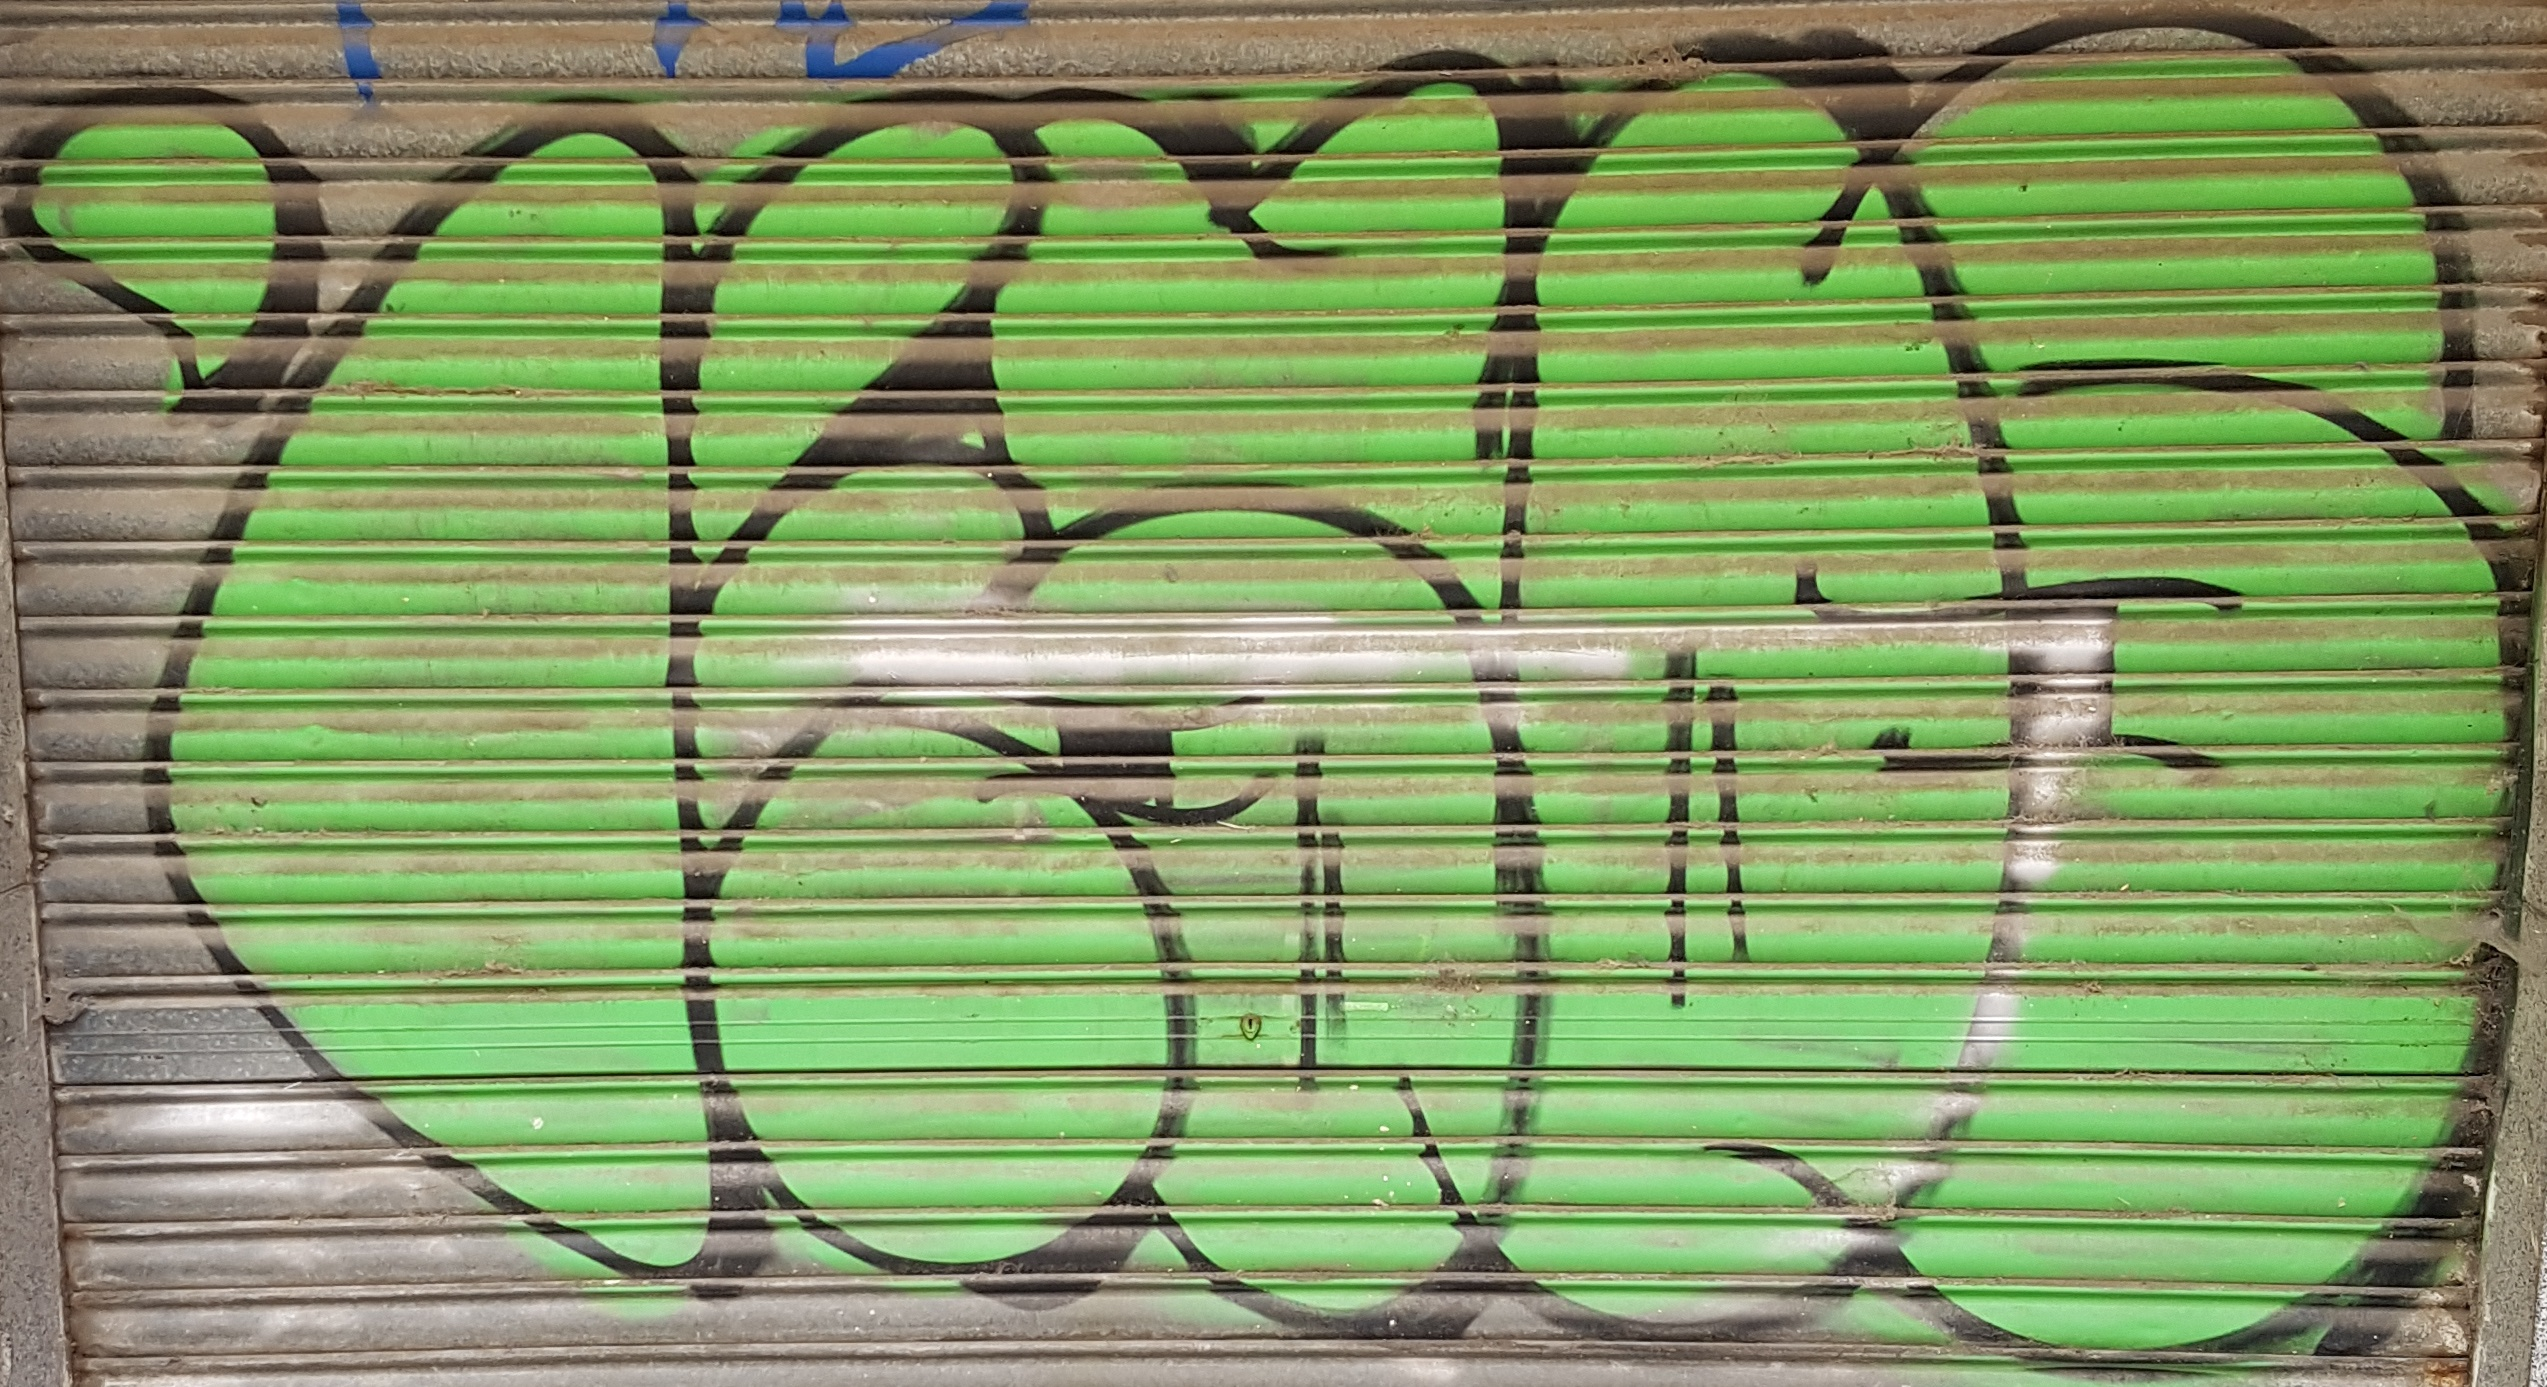
\includegraphics[height=1.3cm,width=2.4cm,keepaspectratio]{figures/style_throwup.jpg} & \textit{throw-up} & Nombre en letras redondeadas, normalmente con dos colores (contorno y relleno) y ejecución veloz. \\ \hline
    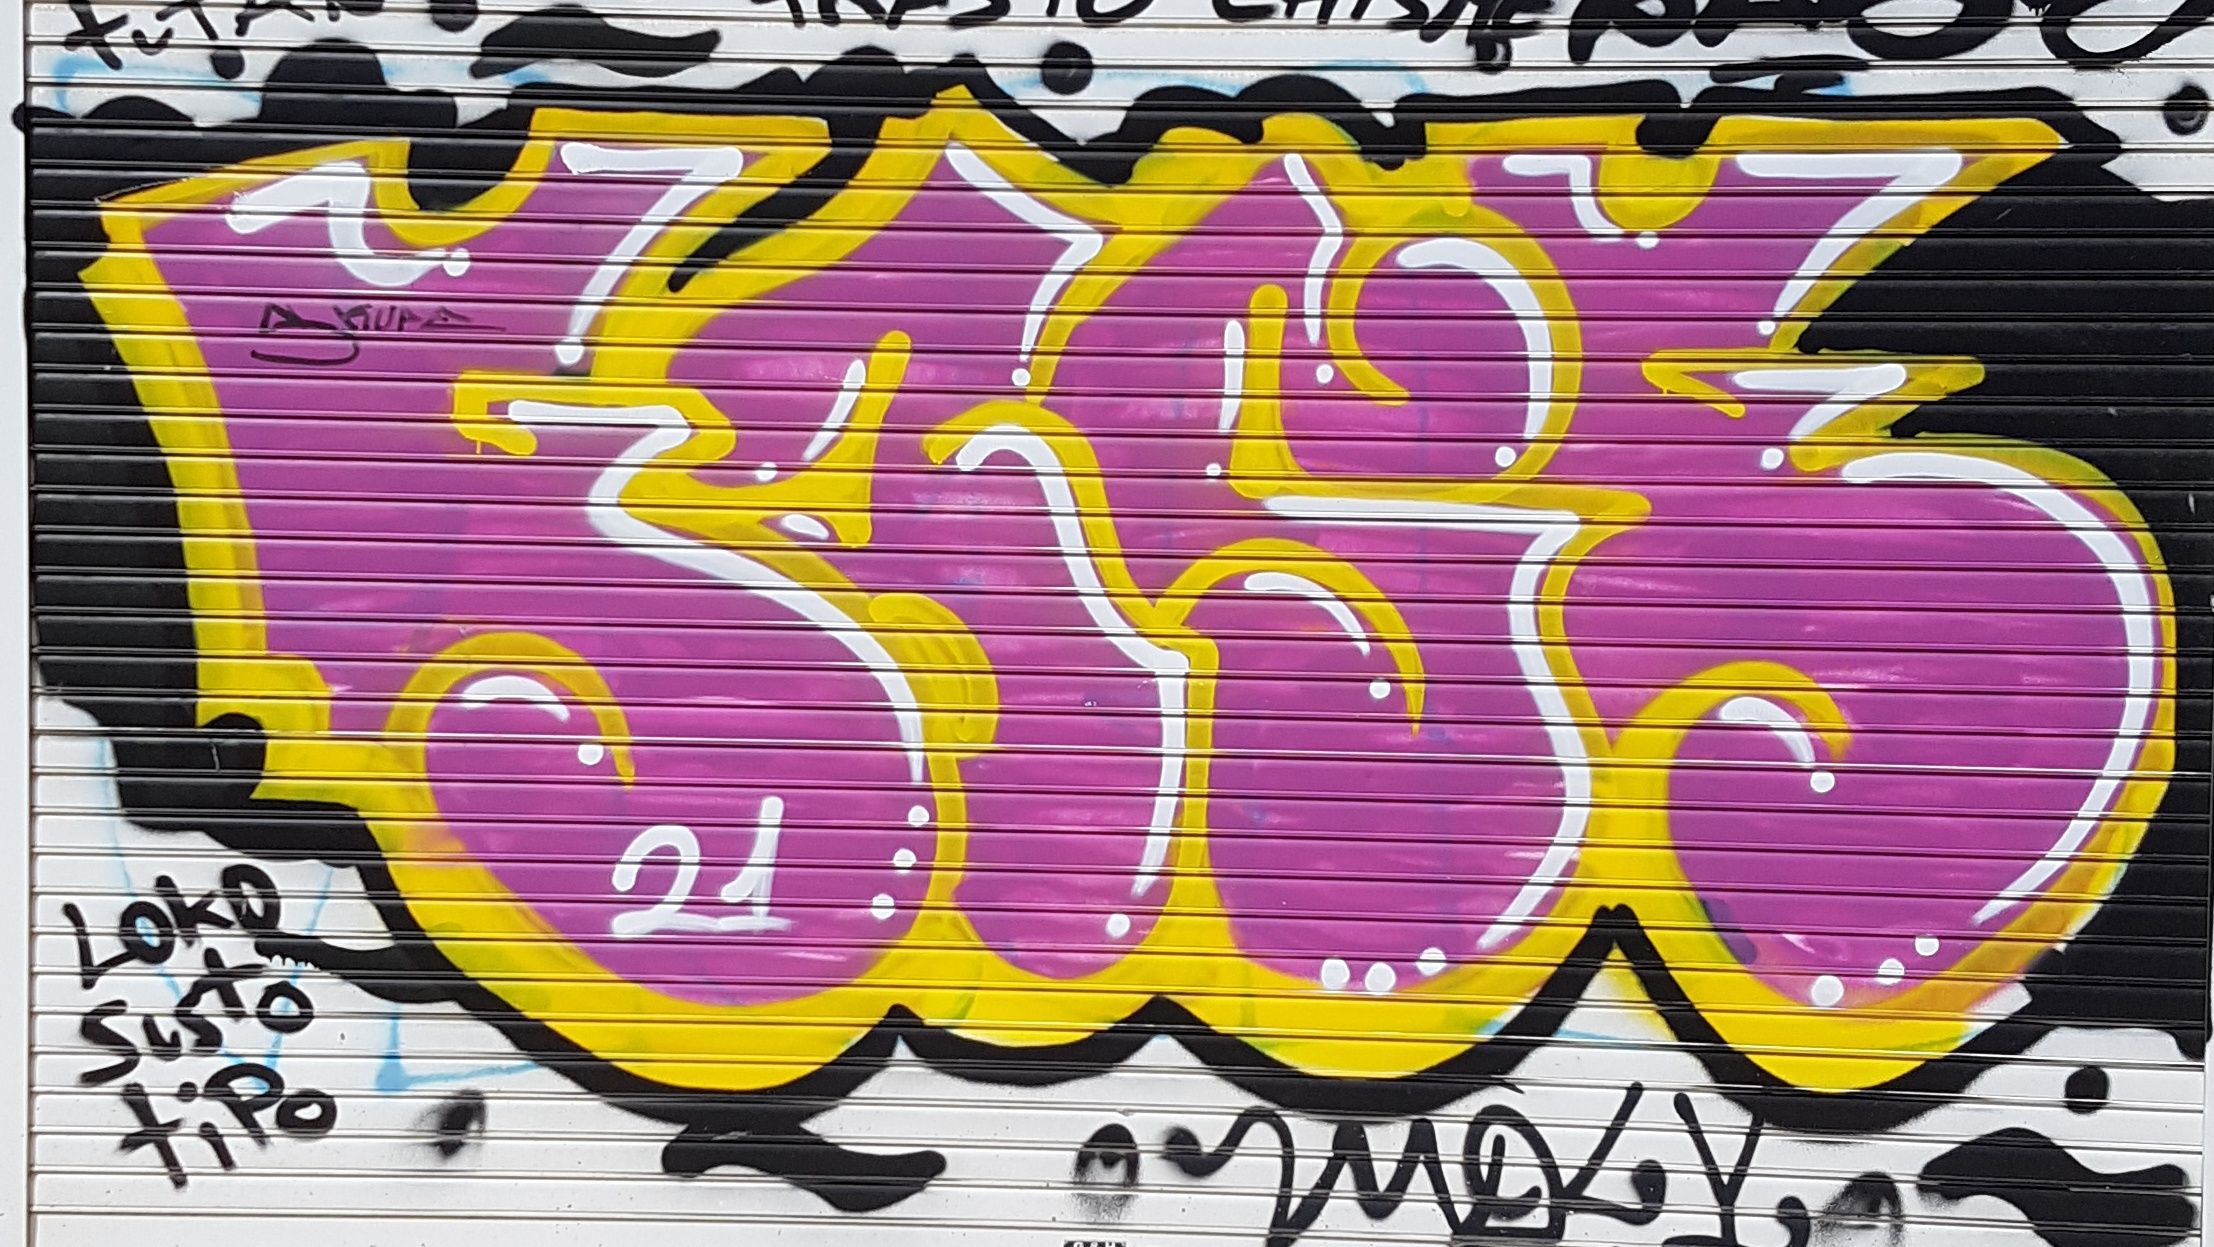
\includegraphics[height=1.3cm,width=2.4cm,keepaspectratio]{figures/style_piece.jpg} & \textit{piece} & Obra elaborada, multicolor y con letras complejas, sombreados y mayor inversión de tiempo. \\ \hline
    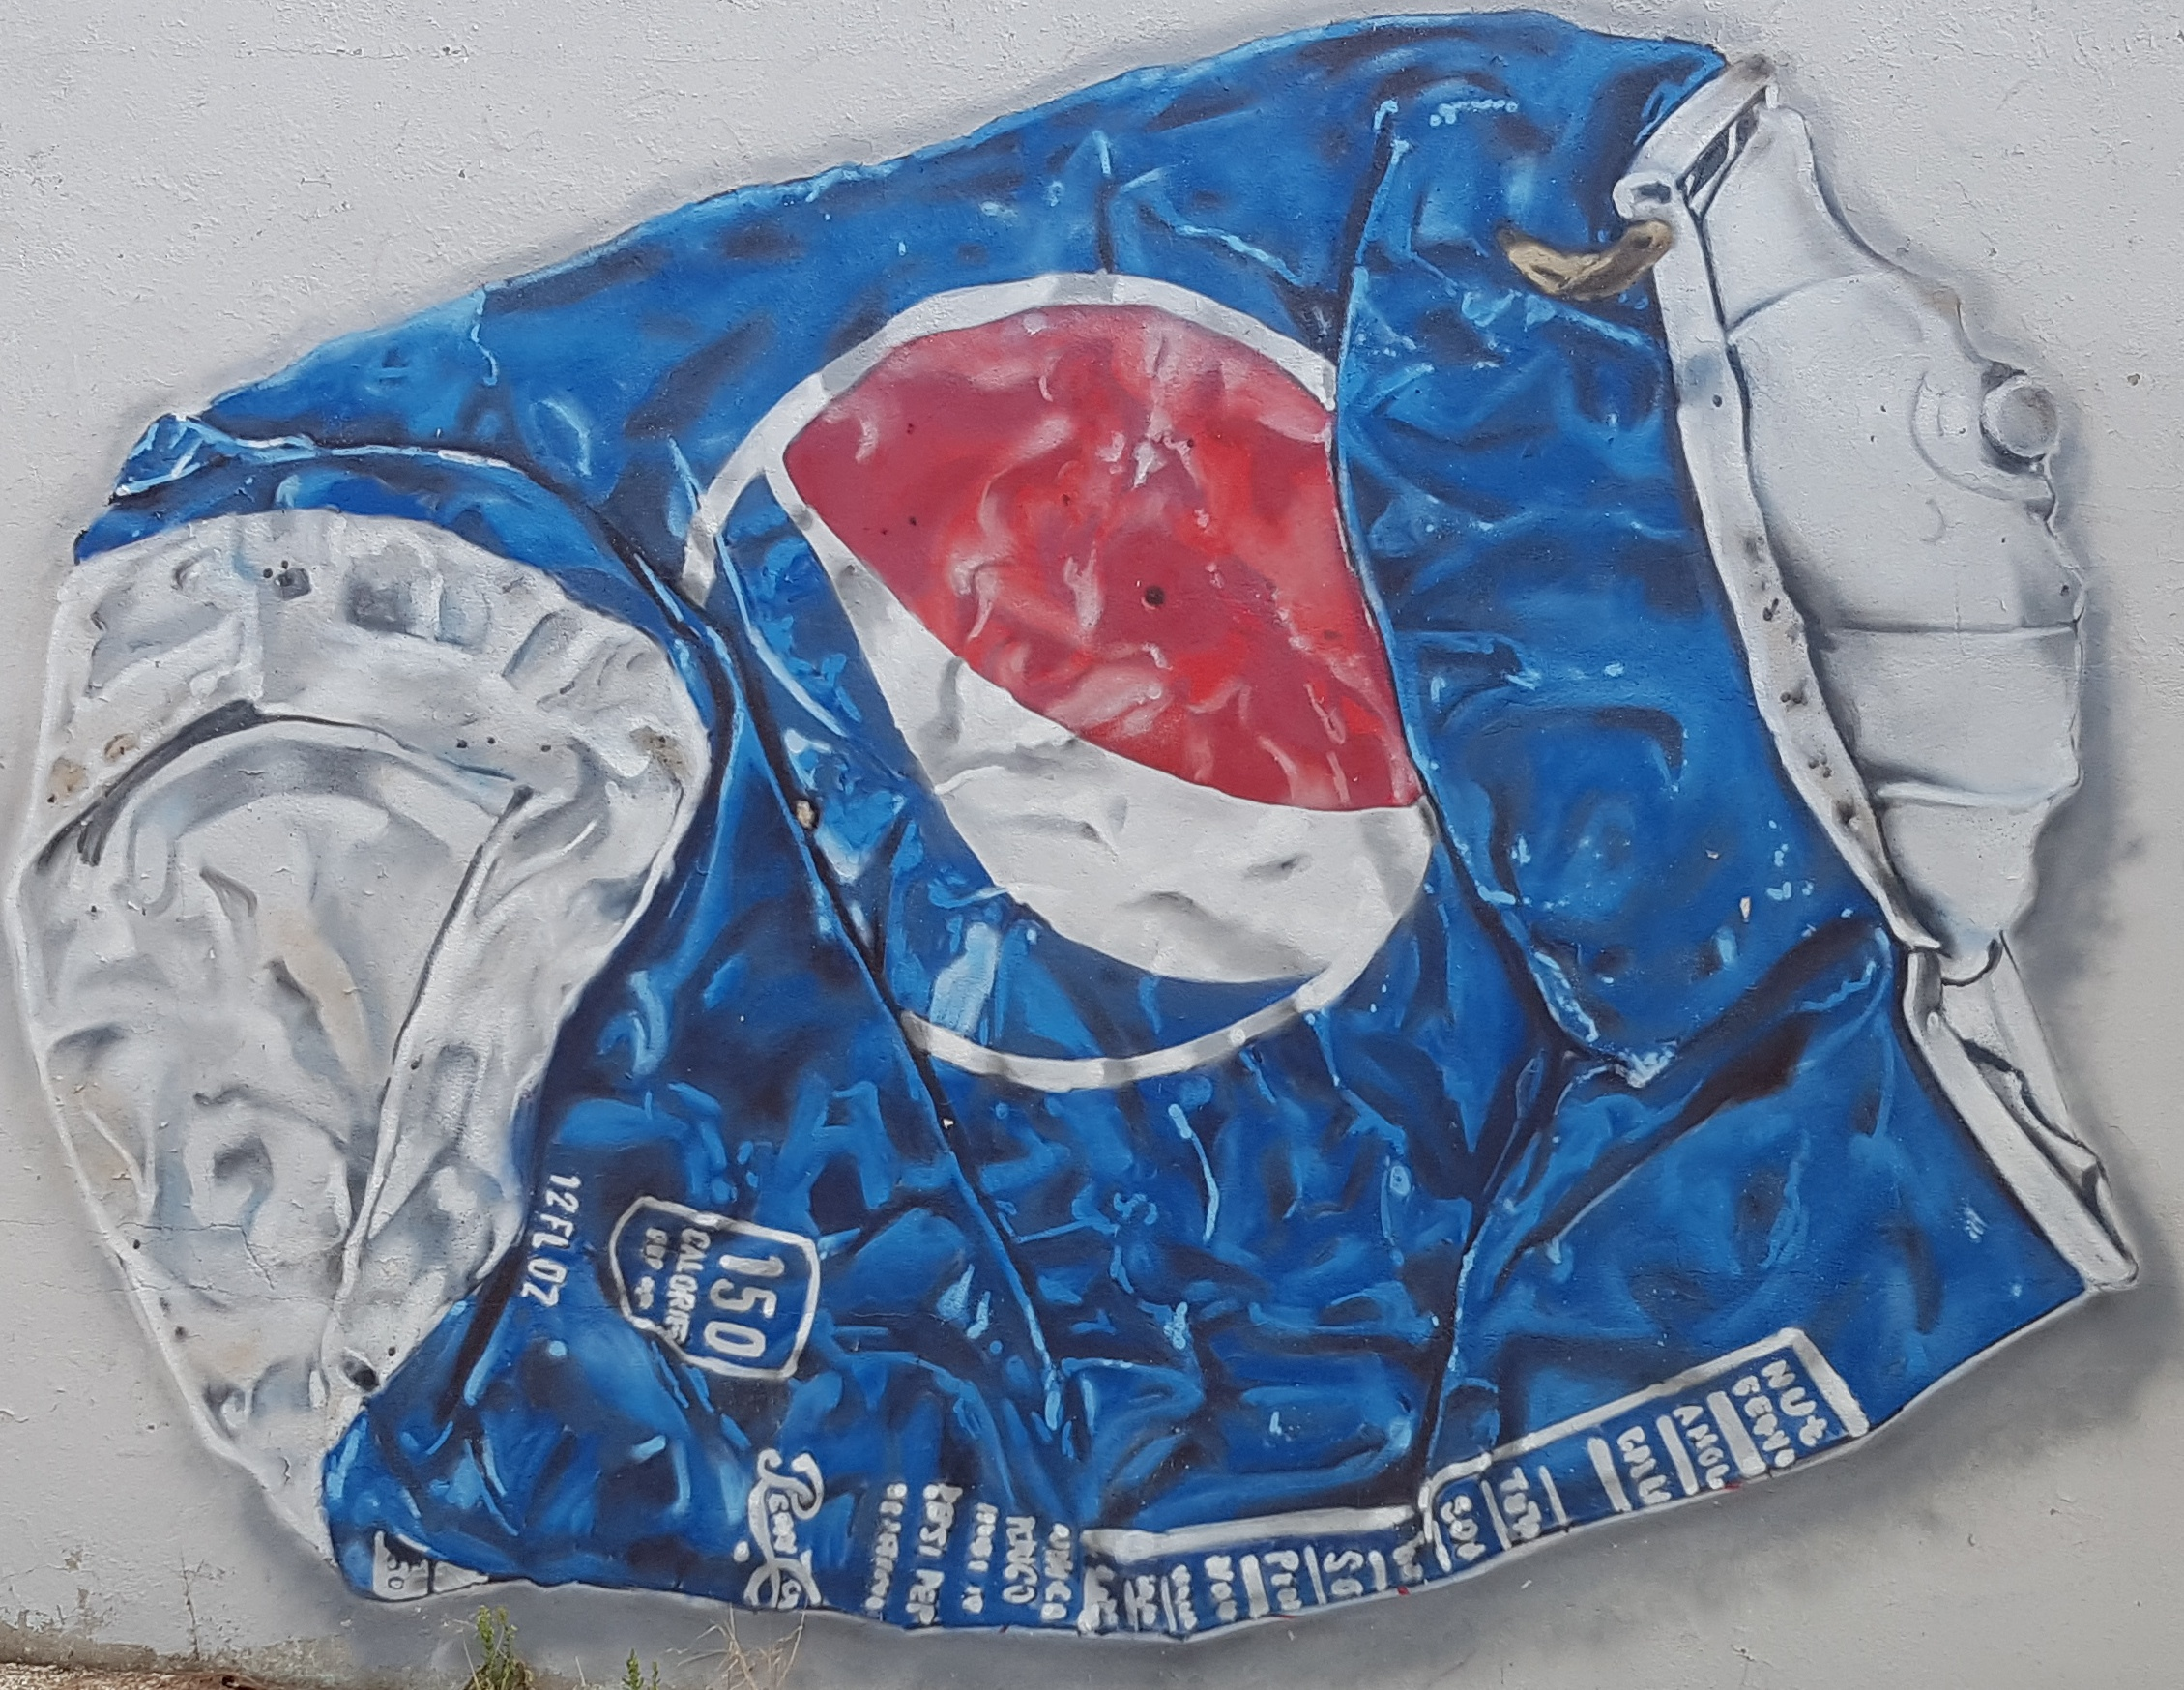
\includegraphics[height=1.3cm,width=2.4cm,keepaspectratio]{figures/style_character.jpg} & \textit{character} & Figura o personaje ilustrado en lugar de letras, a menudo acompañando a otras categorías. \\ \hline
  \end{tabular}
  \caption[Categorías estilísticas etiquetadas]{Categorías estilísticas etiquetadas, con un recorte de ejemplo y su definición.}
  \label{tab:estilos-definiciones}
\end{table}

\begin{table}[h!]
  \centering
  \begin{tabular}{|l|l|l|r|} \hline
    \textbf{Subconjunto} & \textbf{Propósito} & \textbf{Procedencia} & \textbf{Tamaño} \\ \hline
    Estilo (entr.) & Cabezas de estilo & StopGrafiti + Salamanca & $385$ \\ \hline
    Estilo (eval.) & M. Extrínsecas & Banco completo & $294$ \\ \hline
    Autoría (entr.) & Cabezas de autoría & StopGrafiti & $321$ \\ \hline
    Autoría (eval.) & M. Extrínsecas & Salamanca & $185$ \\ \hline
    Detección & Ajuste del detector & Ambos bancos & $447$ \\ \hline
    No superv. & Agrupamiento & Salamanca (disjunto) & $6416$ \\ \hline
  \end{tabular}
  \caption[Subconjuntos etiquetados empleados]{Subconjuntos empleados (en recortes, salvo detección y no
  supervisión, en imágenes). Los recortes de entrenamiento nunca se solapan con
  los de evaluación.}
  \label{tab:subconjuntos}
\end{table}

\subsection{Marco conceptual}
\label{subsec:conceptos}
Cada grafiti se representa mediante un \textit{embedding}, un vector de
características obtenido con modelos preentrenados sobre tareas de visión
generalistas; para las CNN de clasificación (ResNet, VGG) se accede a la
representación latente eliminando las capas finales, mientras que DINOv2 o CLIP
ya devuelven el vector directamente. La similitud se mide con distancia
euclidiana o coseno; ambas coinciden cuando los vectores están normalizados a
norma unitaria ($L_2$), por lo que CLIP, MobileNetV3 y las cabezas de dominio
(que normalizan su salida) usan coseno y el resto, euclidiana.

\subsubsection{Búsqueda por similitud.}
\label{subsubsec:tools-similarity-search}
Se consideran dos enfoques: una búsqueda exacta por fuerza bruta sobre SQLite,
que garantiza el vecino más cercano real a costa de un coste lineal por
consulta, y un índice aproximado HNSW~\cite{malkov_efficient_2018} sobre
PostgreSQL (\textit{pgvector}), mucho más eficiente pero sin garantía de
exactitud. Cuando hay etiquetas se evalúa la calidad de recuperación con P@$k$,
R@$k$, el rango recíproco medio (MRR) y la precisión media promedio (MAP@$k$).

\subsubsection{Agrupamiento y reducción de dimensionalidad.}
\label{subsubsec:agrupamiento}
Se cubren los principales paradigmas de agrupamiento: centroides
(K-medias~\cite{arthur_k-means_2007}), densidad
(DBSCAN~\cite{ester_density-based_1996},
OPTICS~\cite{ankerst_optics_1999},
HDBSCAN~\cite{campello_density-based_2013}), jerárquicos, espectrales,
probabilísticos (GMM~\cite{dempster_maximum_1977}) y \textit{affinity
propagation}~\cite{frey_clustering_2007}. Los métodos de densidad toleran formas
arbitrarias y ruido pero se degradan en alta dimensión, lo que motiva una etapa
previa de reducción ante la maldición de la
dimensionalidad~\cite{aggarwal_surprising_2001}: lineal
(PCA~\cite{jolliffe_principal_2002}) o no lineal
(Kernel PCA, Isomap~\cite{tenenbaum_global_2000},
UMAP~\cite{mcinnes_umap_2020}). La selección del número de clústeres sin
etiquetas se resuelve con heurísticas (método del codo, BIC) en K-medias, DBSCAN
y GMM.

\subsubsection{Métricas de evaluación.}
\label{subsubsec:metricas}
La calidad se valora con dos familias de métricas. Sobre el banco sin etiquetar
se emplean métricas \emph{intrínsecas}, calculadas directamente sobre los
\textit{embeddings}: el coeficiente de
silueta~\cite{rousseeuw_silhouettes_1987} (cohesión vs.\ separación, $\uparrow$),
el índice de Calinski--Harabász~\cite{calinski_dendrite_1974} (razón de
varianzas inter/intracluster, $\uparrow$) y el de
Davies--Bouldin~\cite{davies_cluster_1979} (peor caso de
dispersión/separación, $\downarrow$). Como algunos algoritmos etiquetan puntos
como ruido, estas se complementan con tres indicadores estructurales: número de
clústeres, fracción de ruido y coeficiente de variación del tamaño de los
clústeres, que permiten distinguir un buen agrupamiento de uno que descarta los
puntos difíciles. Sobre los recortes etiquetados por estilo o autoría se calculan
métricas \emph{extrínsecas} que usan la verdad de referencia: el índice de Rand
ajustado (ARI), la información mutua normalizada (NMI) y la F1 por pares.

\subsection{Catálogo de componentes}
\label{subsec:configuraciones}
Todos los modelos de extracción se usan congelados. La
tabla~\ref{tab:embedding-models} resume los extractores integrados (arquitectura,
dimensión de salida y preentrenamiento), la
tabla~\ref{tab:clustering-algos} los agrupadores y sus hiperparámetros clave (la
columna «Auto.\ $k$» indica cuáles estiman su hiperparámetro principal cuando no
se declara, según \ref{subsubsec:hiperparam-auto}) y la
tabla~\ref{tab:reduction} las técnicas de reducción. La persistencia de los
\textit{embeddings} se abstrae tras una interfaz común con dos \textit{backends}:
SQLite (sin servicios externos, búsqueda lineal exacta) y PostgreSQL con
\textit{pgvector} (búsqueda en el SGBD, con índice HNSW opcional). El índice HNSW
de \textit{pgvector} impone un límite de 2000 dimensiones, no aplicable a
ResNet50 e InceptionV3 (2048) ni a VGG16 (4096).

\begin{longtable}{|p{3.2cm}|p{3.8cm}|c|p{4.2cm}|} \hline
  \textbf{Modelo} & \textbf{Arquitectura} & \textbf{Dim.} & \textbf{Preentrenamiento} \\ \hline
  ResNet50~\cite{he_deep_2015} & CNN residual & $2048$ & ImageNet \\ \hline
  VGG16~\cite{simonyan_very_2015} & CNN profunda & $4096$ & ImageNet \\ \hline
  InceptionV3~\cite{szegedy_rethinking_2015} & CNN multi-rama & $2048$ & ImageNet \\ \hline
  MobileNetV3~\cite{howard_searching_2019} & CNN ligera & $1280$ & ImageNet \\ \hline
  DINOv2 ViT-S/14~\cite{oquab_dinov2_2024} & \textit{Transformer}~\cite{dosovitskiy_image_2021} & $384$ & Autosupervisado (LVD-142M) \\ \hline
  CLIP ViT-B/32~\cite{radford_learning_2021} & \textit{Transformer} & $512$ & Imagen-texto (WIT) \\ \hline
  YOLO11 (n/m)~\cite{ultralytics_ultralytics_2024} & Detector \textit{one-stage} & $256$--$512$ & COCO \\ \hline
  \caption{Modelos de extracción de características integrados.}
  \label{tab:embedding-models}
\end{longtable}

\begin{longtable}{|l|l|c|} \hline
  \textbf{Algoritmo} & \textbf{Hiperparámetros principales} & \textbf{Auto. $k$} \\ \hline
  K-medias~\cite{arthur_k-means_2007} & $n\_clusters$ & sí \\ \hline
  DBSCAN~\cite{ester_density-based_1996} & $\epsilon$, $min\_samples$ & sí ($\epsilon$) \\ \hline
  HDBSCAN~\cite{campello_density-based_2013} & $min\_cluster\_size$ & no requiere \\ \hline
  OPTICS~\cite{ankerst_optics_1999} & $min\_samples$, $max\_eps$ & no requiere \\ \hline
  Aglomerativo~\cite{mullner_modern_2011} & $n\_clusters$, $linkage$ & no \\ \hline
  Espectral~\cite{ng_spectral_2001} & $n\_clusters$, afinidad & no \\ \hline
  GMM~\cite{dempster_maximum_1977} & $n\_components$, covarianza & sí \\ \hline
  \textit{Affinity Propagation}~\cite{frey_clustering_2007} & $damping$, $preference$ & no requiere \\ \hline
  \caption{Algoritmos de agrupamiento implementados.}
  \label{tab:clustering-algos}
\end{longtable}

\begin{longtable}{|l|l|l|} \hline
  \textbf{Técnica} & \textbf{Tipo} & \textbf{Parámetros principales} \\ \hline
  Identity & --- & --- \\ \hline
  PCA~\cite{jolliffe_principal_2002} & Lineal & $n\_components$ \\ \hline
  Kernel PCA~\cite{scholkopf_nonlinear_1998} & No lineal & $n\_components$, \textit{kernel} \\ \hline
  Isomap~\cite{tenenbaum_global_2000} & No lineal & $n\_components$, $n\_neighbors$ \\ \hline
  UMAP~\cite{mcinnes_umap_2020} & No lineal & $n\_components$, $n\_neighbors$, $min\_dist$ \\ \hline
  \caption{Técnicas de reducción de dimensionalidad implementadas.}
  \label{tab:reduction}
\end{longtable}

\subsection{Extensiones específicas para grafiti}
\label{subsec:extras}

\subsubsection{Segmentador YOLO.}
\label{subsubsec:segmentador}
La segmentación localiza los grafitis dentro de la fotografía para que el
extractor opere sobre los recortes en lugar de la escena completa. Se implementan
dos variantes: una identidad (imagen completa) y un detector
YOLO~\cite{ultralytics_ultralytics_2024}, oficial o ajustado sobre grafiti, que
detecta las cajas, fusiona las solapadas y adyacentes (con una salvaguarda que
rechaza fusiones que cubran una fracción excesiva de la imagen), aplica un margen
configurable y, opcionalmente, trunca a las $K$ detecciones de mayor confianza.
El detector se evalúa con precisión, \textit{recall} y mAP a distintos umbrales
de IoU, y se ajusta sobre el subconjunto anotado disjunto del de evaluación.

\subsubsection{Cabezas de proyección ajustadas al dominio.}
\label{subsubsec:cabezas}
Para acortar la distancia entre las representaciones generalistas y el dominio
del grafiti se sigue un esquema de \textit{transfer
learning}~\cite{pan_survey_2010,howard_universal_2018}: el \textit{backbone} se
mantiene congelado y solo se entrena una cabeza ligera
(Lineal~$\rightarrow$~ReLU~$\rightarrow$~Lineal) cuya salida se normaliza a norma
unitaria ($L_2$), de modo que sea comparable por distancia coseno. Se entrenan
cuatro cabezas (autoría y estilo $\times$ MobileNetV3 y DINOv2) que proyectan a
$128$ dimensiones (DINOv2 $384\to128$, MobileNetV3 $1280\to128$) y se añaden al
catálogo de extractores.

\subsection{Entorno de ejecución}
\label{subsec:entorno}
Los experimentos se realizaron en un portátil con CPU AMD Ryzen 7 5800H, GPU
NVIDIA GeForce GTX 1650 y 16~GB de RAM. El entorno se basa en Python 3.14
gestionado con \texttt{uv}, con PyTorch 2.10.0 (fijado de forma exacta) como
dependencia nuclear, junto a \textit{open-clip-torch}, \textit{ultralytics},
\textit{scikit-learn}, \textit{umap-learn} y \textit{SQLAlchemy} con
\textit{pgvector}, entre otras.
